\documentclass[sigart]{acmart_mod} %use acmart_mod for handin
% NOTE: To make the documnet anonymous, use the command \documentclass[sigconf, anonymous]{acmart}
%
%% \BibTeX command to typeset BibTeX logo in the docs
\AtBeginDocument{%
	\providecommand\BibTeX{{%
		\normalfont B\kern-0.5em{\scshape i\kern-0.25em b}\kern-0.8em\TeX}}}

\usepackage{lipsum}
\usepackage{graphicx}
\usepackage{tikz}
\usetikzlibrary{arrows.meta}
%% Rights management information.  This information is sent to you
%% when you complete the rights form.  These commands have SAMPLE
%% values in them; it is your responsibility as an author to replace
%% the commands and values with those provided to you when you
%% complete the rights form.
\copyrightyear{2024}
\acmYear{2024}
\setcopyright{rightsretained}
\acmISBN{N/A}
\acmDOI{N/A}

%% These commands are for a PROCEEDINGS abstract or paper.
\acmConference[CMPUT 302 '24: Illumia Labs]{}{January 2024}{Edmonton AB}

% shorthand for ualberta definition
\newcommand{\ualberta}{
	\affiliation{%
	  \institution{the University of Alberta}
	  \city{Edmonton}
	  \state{Alberta}
	  \country{Canada}
	}
}

\begin{document}
	%%
	%% The "title" command has an optional parameter,
	%% allowing the author to define a "short title" to be used in page headers.
	\title{Illumia Labs \textit{Scenario Builder} Discount Evaluation}
	
	%% The "author" command and its associated commands are used to define
	%% the authors and their affiliations.
	%% Of note is the shared affiliation of the first two authors, and the
	%% "authornote" and "authornotemark" commands
	%% used to denote shared contribution to the research.
	\author{Ayrton Chilibeck}
	\authornote{All authors contributed equally to this research, and are listed in alphabetical order for simplicity}
	\email{achilibe@ualberta.ca}
	\ualberta

	\author{Eric Kim}
	\authornotemark[1]
	\email{dek@ualberta.ca}
	\ualberta

	\author{Yu Liu}
	\authornotemark[1]
	\email{yliu30@ualberta.ca}
	\ualberta
	
	\author{Vedant Talati}
	\authornotemark[1]
	\email{vtalati@ualberta.ca}
	\ualberta

	\author{Marcus Wilson}
	\authornotemark[1]
	\email{mawilso1@ualberta.ca}
	\ualberta

	%%
	%% By default, the full list of authors will be used in the page
	%% headers. Often, this list is too long, and will overlap
	%% other information printed in the page headers. This command allows
	%% the author to define a more concise list
	%% of authors' names for this purpose.
	\renewcommand{\shortauthors}{Chilibeck, Kim, Liu, Talati, Wilson}
	
	%%
	%% The abstract is a short summary of the work to be presented in the
	%% article.

	\maketitle
	
\section{Introduction}
We assess Illumia Lab's \textit{Scenario Builder} to identify areas for enhancement and offer a short-term development roadmap. We address issues in UI, system functionality, and program documentation, drawing upon Human-Computer Interaction (HCI), Gestalt, and CRAP design principles. Our solutions align with established HCI research, color theory, and user experience insights.
\section{System Flaws}\label{sec:flaws}
Throughout our investigation and utilization of the system, we identified issues in the UI, program functionality, and documentation. We highlight the key findings in the subsequent sections.
\subsection{UI}

Our examination of the UI primarily addresses cosmetic issues, yet the current software state hinders effective user interaction. The layout fails to efficiently display scene information, and scene transitioning demands excessive user effort. Moreover, clear indications of appropriate user actions are lacking throughout the scene-building process.

\subsubsection{Color Scheme}

The existing color scheme (Purple (\verb|#07012F|), Blue (\verb|#0191FD|), and Red (\verb|#FC5C00|)) is visually straining. Research indicates that prolonged exposure to red and purple hues can be taxing for users~\cite{jonesHumancomputerInteractionDesign1989}. Some users may prefer alternative color schemes, and implementing a light and dark mode could enhance interface versatility. Additionally, the use of red to signify the program's desired state among multiple choices may confuse users, given red's association with 'negation' or 'emergency' decisions.

\subsubsection{Tab Display}

The current tab display in the scene builder inadequately communicates the program's status to users. Tabs for each scene lack context regarding their purpose or contained information. Although the preview pane partially addresses this issue, the scene-graph representation lacks clarity regarding scene relationships.

\subsubsection{Preview Pane}

The preview pane suffers from poor alignment and lacks dynamic screen resizing, diminishing the utility of presented data, especially for mobile and resizable web pages.

\subsubsection{Ease of Use}

Constructing a scene currently requires a minimum of 9 clicks. While the '3-click rule' has been debunked~\cite{ThreeclickRule2023}, ensuring ease of information access remains crucial in design. Recent research on 'Interaction Elasticity' underscores the importance of minimizing unnecessary interactions~\cite{experienceInteractionElasticity}. Presently, the scene builder imposes excessive interaction burdens on users through these clicks.

\subsection{Functionality}

The website currently lacks implementation of several usability-enhancing features, impacting user experience. We outline the affected systems below.

\subsubsection{Saving}

At present, the system does not support scene saving or the ability to resume work on previously saved scenes. This limitation hampers users' ability to create meticulously crafted scenes.

\subsubsection{Avatar}

The inclusion of an avatar in scene development appears superfluous, as its necessity is not reflected in the builder's stated requirements or business logic. Observing the intention to include the avatar, we assume that this feature is not yet implemented.

\subsection{Documentation}

Overall, the builder suffers from inadequate documentation. Many terms and software interactions remain unexplained, decreasing user understanding of the program's functionality.

\section{Remediations}\label{remediations}
We propose several solutions to the problems mentioned above that will improve the usability of the application and touch on additional, smaller problems that we neglect to mention in this report, but are nonetheless important.

\subsection{UI}
\begin{figure}
  \begin{center}
  \includegraphics[scale=0.4]{media/sidebar.png}
  \end{center}
\caption{A prototype sidebar navigation system.}\label{fig1}
\end{figure}
We suggest a sidebar-based UI such as pictured in Figure \ref{fig1}. This UI paradigm will provide the user with more information on any given scene in the program and allow the user to recognize the full state of the program at a glance without wading through screen after screen of data.

When combined with an information page for the selected screen (or the graph view of connections between scenes), we can give the user a more granular view of the data. It is important to note that this type of modification is an overhaul of the frontend design for the website, so the transition will not be easy but the application of this type of UI is well-loved in modern UI design~\cite{YourConnectedWorkspace} \cite{SupabaseOpenSource} \cite{FlutterBuildApps}. Adding the flexibility for the user to navigate to any scene in a single click will then reduce useless interaction with the program, bettering the user experience.

This type of UI will also make user error handling more visible to the user. Instead of using the single exclamation point, we can highlight all the fields' invalid data on the associated page and provide a clear message to the user concerning the nature of their violations all on one screen. We can also highlight the issues in all scenes by highlighting nodes on the sidebar as required. This way, the user does not need to chase every bug individually and can rather see where every bug is without having to perform trial-and-error modifications.

\subsubsection{The Scenarios Folder}
You will notice in the mockup that we have added a scenarios folder, this serves to give the user a space to switch between different scenarios they are beginning to develop and possibly to store other scene elements they use frequently. This will require the implementation of the saving system, but will improve the user's ability to reuse gode as required.

\subsubsection{Log Out}
The sidebar also contains a Log-Out button, it is assumed that eventually the avatar will be associated with the user to create some kind of account for the user to log in and out with. This would be an easy way to implement this feature.

\subsubsection{The Scenario Page}
\begin{figure*}
  \begin{center}
	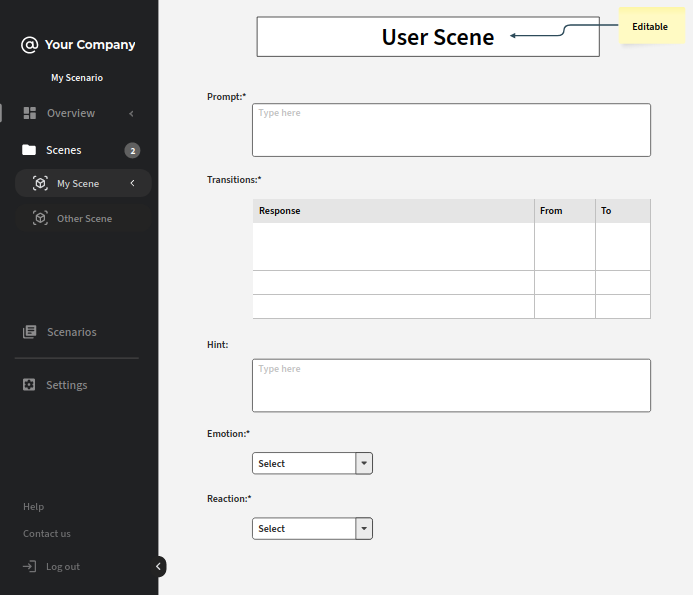
\includegraphics[scale=0.4]{media/Scene_Page.png}
  \end{center}
\caption{A mockup of a scene page for editing individual scenes in the program}\label{fig2}
\end{figure*}
The accompanying scenario page shown in Figure \ref{fig2} will give the user the option to input all necessary data and efficiently view all of their options. This will provide a visual interface for the user to modify their scene without added interaction.

Additionally, there is the option to outline the elements in red or some other colour to indicate a non-conforming piece of data. In the tab-like display, the user is not aware of the exact location of flaws in their data.

We could also implement a dropdown in the sidebar for each scene that gives a short summary of the data entered and can also indicate errors in the data entry. This will give users an even more general view of their scene.

\textbf{Note}: We are unsure of the difference between the emotion and reaction elements. The two descriptions seem to be linked, and as such we wonder if the program could eliminate one or the other.

\subsection{Functionality}
With the implementation of a sidebar navigation paradigm, we can eliminate the need for a lot of the confusing actions that were present in the tab layout. This includes the arrows above the tabs and the delete button (which could now be placed on the sidebar element or in its dropdown menu), as well as a myriad of alignment problems. Now the data has one single point of control that can be stored as one object for manipulation and viewing.

\subsubsection{Saving}
We suggest that the 'Scenarios' folder hold all of the user's stored scenarios. The user's account status and data could be put on a ribbon across the top of the screen, potentially containing links to the other tools Illumia Labs licenses.

This would not only allow users to store their previously constructed scenarios and use template ideas, but also encourage the use of the entire ecosystem developed by Illumia Labs.

\subsubsection{Avatar}
We further suggest that the avatar become part of an account creation process and eliminate the functionality from the scenario builder itself. This would eliminate the confusion caused by the opening scene both asking for an avatar and allowing them to continue without one.

In addition, removing the avatar creator from the builder allows us to abstract the account away from the business logic in the builder, which will allow better system-level encapsulation.

\subsection{Documentation}

Developing succinct and useful documentation will help the user experience immensely. Currently, it is unclear what the scenario builder does based on the interface. We suggest adding a 'help' icon to present a brief description of what a given element does and pointing the user to a full documentation page if the logic is too complex to describe in a tooltip.

\section{Suggested Roadmap}
Due to the number of distinct changes we proposed and their complexity, we suggest proceeding with the following roadmap in mind:
\begin{itemize}
  \item \textbf{~4-6 weeks} UI Revamp
  \item \textbf{~4-6 weeks} Documentation site
  \item \textbf{~1 week} Integrate the documentation as tooltips and links on the UI
  \item \textbf{~2-4 days} Choose a different colour scheme
  \item \textbf{~4-6 weeks} Add a graph representation of the scenes and their interactions
\end{itemize}
For a total of ~20 weeks of work. We will detail the phases below.

We should note that much of this work can be done collaboratively and in parallel, thus the work cycle should not take the full 20 weeks we estimate.

\subsection{UI Revamp}
We propose changing the UI to reflect our suggestions. This will require making a new landing page and then implementing the business logic and making the appropriate changes to the representation and functionality we described in section \ref{remediations}.

Ideally, this is accompanied by changes in the backend to better reflect the data acquired from the user in their interactions with the program. We will not comment more on the backend due to our lack of exposure.

\subsection{Documentation}
We propose mounting a separate website for documentation using some easily configurable and customizable system such as Docusaurus~\cite{FacebookDocusaurus2024}, GitBook \cite{GitBookKnowledgeManagement}, or Docsify \cite{DocsifyjsDocsifyMagical}. This will need to contain the following sections:
\begin{itemize}
  \item \textbf{Quickstart}: A section to get the user acquainted with the software quickly, exposing them to the most important and relevant features of the program.
  \item \textbf{Introduction}: A section to describe the purpose of the software (possibly pointing to examples of existing systems or your own examples).
  \item \textbf{Documentation}: A section to fully document all features of the site, including individual actions the user can perform and their expected effect. This section may also contain information as to data input requirements and data use and privacy.
\end{itemize}
\subsection{Integrate Documentation}
This consists of linking the documentation created in the previous step and linking it to the correct element associated with the action. This also embodies the creation of tooltips and help buttons as required on every screen. This will allow the user to quickly and efficiently find the answer to their question and increase the usability of the site in general.

\subsection{New Colour Scheme}
Considering the taste of the current colour scheme (relatively dark and cool colours), we suggest implementing a colour scheme of complimentary colours.

\subsection{Graph Representation}
\begin{figure}
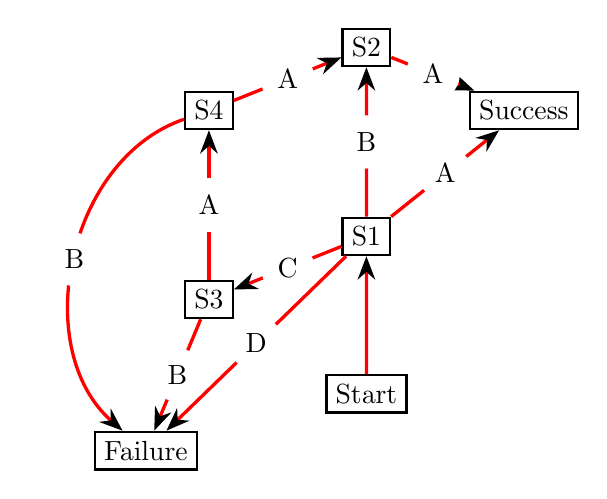
\begin{tikzpicture}[scale=0.8]
\begin{scope}[every node/.style={rectangle,thick,draw}]
    \node (A) at (0,0) {S3};
    \node (B) at (0,3) {S4};
    \node (C) at (2.5,4) {S2};
    \node (D) at (2.5,1) {S1};
    \node (E) at (2.5,-1.5) {Start};
    \node (F) at (5,3) {Success} ;
	\node (G) at (-1, -2.4) {Failure};
\end{scope}

\begin{scope}[>={Stealth[black]},
              every node/.style={fill=white,circle},
              every edge/.style={draw=red,very thick}]
    \path [->] (A) edge node {A} (B);
    \path [->] (B) edge node {A} (C);
    \path [->] (D) edge node {C} (A);
    \path [->] (D) edge node {B} (C);
    \path [->] (A) edge node {B} (G);
    \path [->] (D) edge node {D} (G);
    \path [->] (D) edge node {A} (F);
    \path [->] (C) edge node {A} (F);
    \path [->] (E) edge (D);
    \path [->] (B) edge[bend right=60] node {B} (G);
\end{scope}
\end{tikzpicture}
\caption{A depiction of the relationship between scenes using a graph representation. Adapted from~\cite{tAnswerDrawGraph2015}}\label{fig:scene_graph}
\end{figure}
The graph representation of scenes will serve as a replacement for the preview panel. Instead of providing a text-based representation of the relationships between scenes, consider providing a visual one such as displayed in Figure \ref{fig:scene_graph}. A popular example comes from Obsidian's knowledge graph~\cite{ObsidianSharpenYour}, which contains back-links and grouping to visually demonstrate the relationship between different nodes in the graph.

An automatically generated graph could easily be produced from the data in a scene, but rendering the graph would take some engineering, hence the predicted time allotment.

In addition to allowing the user control over the way their scenes interact and providing more detailed information on the scenario structure, this also adds an option for a new type of node creation that could be done visually in the graph. This, though an interesting idea, leaves a cost-benefit analysis to the reader.

\section{Conclusion}

Throughout this paper, we have highlighted various visual, functional, and documentation deficiencies within the Illumia Labs \textit{Scenario Builder}. Our assessment reveals a user interface that is cumbersome to navigate and characterized by unnecessary interactions, which diminishes program usability. Issues such as color scheme, layout, alignment, and contrast, as well as several Gestalt principles outlined in Section \ref{sec:flaws}, contribute to this usability challenge.

In response, we propose a comprehensive five-step plan to rectify these identified issues, offering potential solutions for each problem. Additionally, we delve into specific UI problems in the appendix and advocate for a complete overhaul of the UI. Our analysis draws from both scholarly literature and prevalent community practices, providing valuable insights to enhance the attractiveness and user-friendliness of the Illumia Labs \textit{Scenario Builder}.
% bibliography data
\bibliographystyle{ACM-Reference-Format}
\bibliography{bibliography}
\end{document}
\endinput
%%
%% End of file `sample-lualatex.tex'.

% LocalWords:  alottment paralell excersized
